
Our method consists of a node embedding algorithm (\emph{Deepwalk}), a greedy clustering algorithm (\emph{K-means}), the modified version of \emph{ddCRP} and the modified version of MCLA. The whole pipeline is described in Figure \ref{fig:pipeline}.

\begin{figure}
    \centering
    \makebox[\textwidth][c]{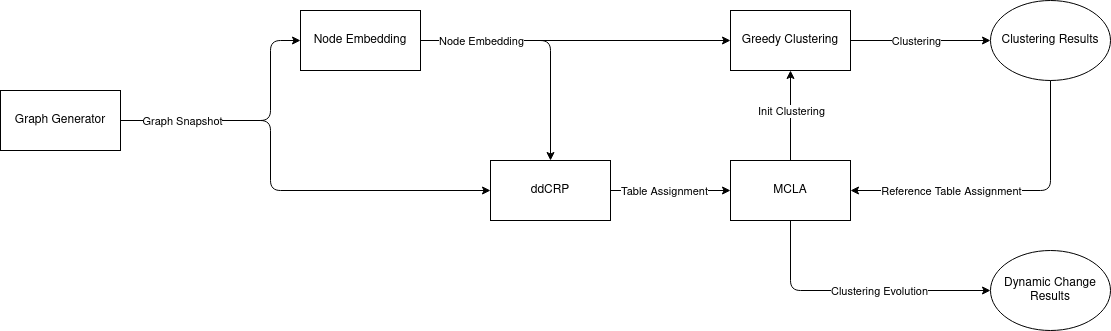
\includegraphics[width=1.4\textwidth]{report/assets/pipeline.png}}
    %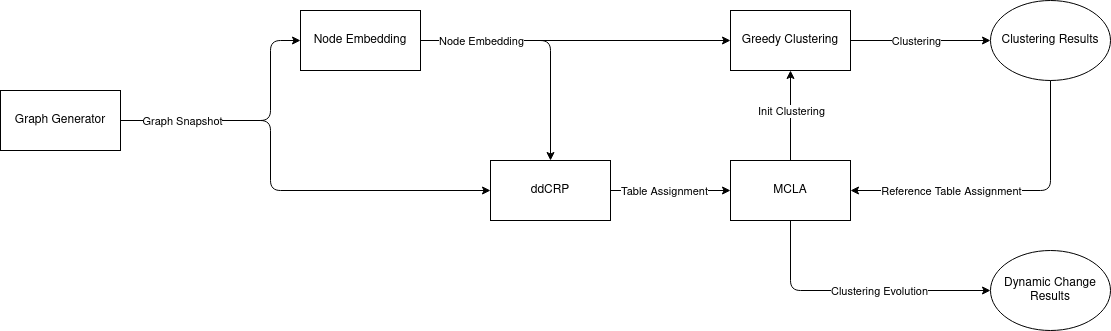
\includegraphics[width=1.2\textwidth]{report/assets/pipeline.png}
    \caption{Algorithm Pipeline}
    \label{fig:pipeline}
\end{figure}

In each iteration, Graph Generator generates graph snapshots. The graph snapshots are then passed to Node Embedding algorithm and \emph{ddCRP}. \emph{ddCRP} then takes the results from Node Embedding to generate a series of table assignments which are the high probability region. The \emph{MCLA} algorithm takes the table assignments from \emph{ddCRP} together with the old clustering result generates a initial clustering. Greedy Clustering algorithm takes the node embedding and the generated initial clustering then produces the final clustering result. At the same time, \emph{MCLA} algorithm produces the clustering evolution by comparing the old clustering result to the new clustering result.



\newpage
\subsection{Node Embedding}

In the node embedding algorithm, we chose \emph{Deepwalk} as the function converting a graph snapshot into a $d$-dimensional representation. In order to handle the weighted graph, we modified the random-walk probability into:

\begin{equation}
    ChooseProbability(v_j | v_i) \propto \left\{
        \begin{array}{ll}
            w(v_i, v_j) \;\;\;\; \text{if $(v_i, v_j) \in E$}\\
            0 \;\;\;\;\;\;\;\;\;\;\;\;\;\;\;\; \text{otherwise}
        \end{array}
    \right.
\end{equation}

Where $w(v_i, v_j)$ is the weight of edge $(v_i, v_j)$. This is equivalent to consider an edge of weight $w$ as $w$ edges.

\newpage
\subsection{\emph{ddCRP}}

Inspired by the work of  David  M.  Blei  and  Peter  I.  Frazier, we extended the Gibbs sampling algorithm on \emph{ddCRP} for graph clustering problem. In the context of graph, we relaxed the Gibbs sampling scheme by limiting the non-zero probabilities only to the vertex in the receptive field. Define $h$-order receptive field by the matrix $A^*_h = (A+I)^h$ where $A$ is the adjacency. The Gibbs sampling scheme is modified to:

\begin{equation}
    P^*(z[i] = j \;|\; (z - z[i]), \alpha, x, G_0) = r(i, j)P(z[i] = j \;|\; (z - z[i]), \alpha, x, G_0)
    \label{eq:p*}
\end{equation}

Where $r(i, j)$ is:

\begin{equation}
     r(i, j) = \left\{
    \begin{array}{ll}
        1 \;\; \text{if $A^*_h(i, j) \neq 0$}\\
        0 \;\; \text{if $A^*_h(i, j) = 0$}\\
    \end{array}
    \right.
\end{equation}

We then defined the decay function $f(i, j)$ as:

\begin{equation}
    f(i, j) = exp(- s(u_i - u_j)^2)
\end{equation}

Where $s \in R^+$ (scale or precision) is a tune-able hyper-parameter which controls the cluster sizes. This formulation can be seen as assuming each vertex is a Gaussian with precision matrix $2sI$, the decay value is hence proportional to the likelihood of the other vertex given the Gaussian.

We assume each cluster distributes according to a Gaussian and choose NIW as the prior. The prior parameters are initialized according to the book \cite{murphy2012machine} (sec 4.6.3.2).

The calculation of $P^*(z[i] = j \;|\; (z - z[i]), \alpha, x, G_0)$ breaks down into. From \ref{eq:p*}, calculate $r(i, j)$ and calculate $P(z[i] = j \;|\; (z - z[i]), \alpha, x, G_0)$ according to \ref{eq:gibbs}. In \ref{eq:gibbs}, calculate the data likelihood term (the first term) with the assumption that cluster points distribute according to a Gaussian (sec Data marginal likelihood).

The algorithm is hence described as below:

\begin{algorithm}[H]
\caption{Node clustering using Gibbs sampling on ddCRP}
\textbf{Input:}\\
    $X \in R^{|V| \times d}$: node embedding\\
    $G = (V, E, w)$: Undirected weighted graph\\
    $s$: decay scale\\
    $T$: Number of iterations\\

\textbf{Output:}\\
    Table assignment at every iteration\\

\textbf{Data Structures:} \\
    $G_C$: customer graph: an unweighted directed graph \\
    $G_T$: customer-table graph: a bipartite graph between customer nodes and table nodes. Each table is associated with a table likelihood calculated based on equation \ref{eq:table_likelihood}\\


\begin{algorithmic}
\State \textbf{Initialization:} table assignment
\For{$t$ = $1$ to $T$}
    \For{$i$ = $1$ to $|V|$}
        \State Unlink vertex $i$ with its parent in $G_C$, Update $G_T$.
        \State Calculate $P^*(z[i] = j \;|\; (z - z[i]), \alpha, x, G_0)$
        \State Random sampling a vertex $j$ according to $P*$
        \State Link vertex $i$ to chosen $j$ in $G_C$, Update $G_T$.
    \EndFor
    \State Record the table assignment at iteration $t$
\EndFor
\end{algorithmic}
\end{algorithm}

It is notably that the calculation of $P^*(z[i] = j \;|\; (z - z[i]), \alpha, x, G_0)$ is reduced from $O(|V|)$ to $O(d_{max}^h)$ where $d_{max}$ is the maximum degree of the graph. Additionally, all calculations can be performed in log-scale that totally avoids the problem of floating-point overflow.

The asymptotic complexity is described as follow. In each iteration, the algorithm performs $n = |V|$ updates. Each update consist of (1) Unlink the source node: $O(log(neighbour size))$, update the table assignment, this consists of (1.1) find the new weakly connected component correspond to the source node after the unlink, since the graph has at most one out-going edge for each node, the time complexity for depth-first search is $O(component size)$, (1.2) verify whether the old parent was included in the new connected component: $O(log(component size))$, in the worst case, split. (1.3) If split, update the table assignment. this step consists of (1.3.1) find the new weakly connected component correspond to the old parent of the source node: $O(component size)$. (1.3.2) update the bipartite graph, (1.3.2.1) link customers to new table: $O(component size)$, (1.3.2.2) update table likelihood: $O(table likelihood)$. (2) For each target node in the receptive field, this multiplies the complexity by $receptive field size$, (2.1) calculate the transition probability, (2.1.1) look up for decay value: $O(1)$, (2.1.2) Check if there is a table join: $O(1)$, in the worst case, there is a table join, calculate the joint table likelihood: $O(component size)$. (2.2) random sampling: $O(receptive field size)$, (2.3) Link the source node: $O(log(neighbourhood size))$ to the target node, update the table assignment, this consists of (2.3.1) check whether there is a table join: $O(1)$, in the worst case, there is a table join, (2.3.2) update the bipartite graph (2.3.2.1) link customers to new table: $O(component size)$, (2.3.2.2) update table likelihood: $O(table likelihood)$. The total time complexity for each update is:

\begin{equation}
    O(table likelihood + receptive field size \times component size)
\end{equation}

Given fixed dimension $d$, the time complexity for $table likelihood$ is in the order of $O(component size)$ (we assumed the floating-point calculation takes a constant time). $receptive field size$ is in the order of $d_{max}^h$ where $d_{max}$ is the maximum degree of the network. $component size$ which is typically chosen before hand. The update time complexity is hence:
\begin{equation}
    O(d_{max}^h \times c)
\end{equation}

\newpage
\subsection{\emph{MCLA}}

Since the trajectory of MCMC algorithm lies on the high probability region, we adopted a cluster ensemble method to combine the results from Gibbs sampling to obtain an average of clustering results. Inspired by the concept of \emph{Meta-Graph}, we designed an clustering ensemble algorithm that is capable to produce informative responses from clustering evolution.

The algorithm is described as below:

\begin{algorithm}[H]
\caption{MCLA}
\textbf{Input:}\\
    $C_0 \subseteq \mathcal{P}(U)$: reference clustering, a family of subsets of U\\
    $C \subseteq \mathcal{P}(U)$: new clustering, a family of subsets of U\\

\textbf{Output:}\\
    $P$: a partition of $U$\\
    Response of new clusters, joined clusters.
    
\begin{algorithmic}

\State{Initialization:} construct meta-graph according to definition \ref{def:meta_graph}
\State{Filtering:} Filter out all disconnected components
\State{Clustering:} Partition the meta-graph.
\State{Voting:} For each node, decide the corresponding meta-cluster.
\State{Response:} A meta-cluster is a new cluster if there is no reference cluster belongs to it. A meta-cluster is a join cluster if there is more than one reference clusters belong to it.
\end{algorithmic}
\end{algorithm}


